\section{Notification Module}
\subsection{Overview}
The notifications module provides notifications to system users regarding particular system updates that a user would like to be notified about through some medium external to the application. 
\subsection{External Interface Requirements}
This section gives a detailed description of the system interfaces, hardware interfaces, software interfaces as well as communication interfaces.
\subsubsection{System Interfaces}
\begin{itemize}
	\item The notification module will interface with any subsystem or module that wishes to send out notifications to users. The subsystem requesting for users to be notified is modelled as the Notifying Module. The Notifying module will interface with the Notification Module through the setState() function to send a notification request. 
	
	\item The notification module will interface with the User module in order to sufficiently dispatch notifications. Each instance of the Notifier class will maintain a list of attached users and will send notifications through the notify() function.
\end{itemize}

\subsubsection{User Interfaces}
\begin{itemize}
	\item The system will dispatch notifications in the form of an \textbf{SMS} to the appropriate users. The SMS will contain the content of the notification and the interface will depend on the user's device.
	
	\item The system will dispatch notifications in the form of an \textbf{email} to the appropriate users. The email will have an appropriate subject and will contain the content of the notification. The interface will depend on the mail application used by the user.
	
	\item The system will dispatch notifications in the form of \textbf{Push Notifications}.  push notification will contain a title, content as well as a timestamp. The interface will depend on the user's operating system. 
\end{itemize}

\subsubsection{Hardware Interfaces}
The Notification Module does not have any explicit hardware interfaces

\subsubsection{Software Interfaces}
  \begin{itemize}
  	\item The notification module will communicate with the database in order to get the details of users to be notified.
  \end{itemize}
  
\subsubsection{Communication Interfaces}
	\begin{itemize}
		\item The notification module will need to communicate with an Email API when sending out emails to users
		\item The notification module needs to interface with the SMS Manager API to send SMS's to users.
		\item The notification module will interact with the Operating system push notification service (OSPNS) to allow users to receive push notifications.
	\end{itemize}
	
\subsection{Performance Requirements}
Notifications should be able to perform and guarantee message delivery under high volumes, allow real time notifications to be received and have good network access for this purpose. 

\subsection{Design Constraints}
The notifications must be:
\begin{itemize}
	\item Visually appealing and easy to read, have a gamification point of view
	\item Support viewing on different sizes of device screens
	\item Support colour for all devices
	\item Being able to integrate easily with notification providers
\end{itemize}


\subsection{Software System Attributes}
\subsubsection{Reliability}
The system should make use of a queue to send notifications, so that no messages can get lost on the way and must guarantee that the notification must be delivered.
Notifications should be authentic and be able to verify that delivery of the notification.

\subsubsection{Security}
The sending of the notifications must be secure using proper SMTP setup with SSL encryption for emails, and a authentic SMS provider validated by the WASPA, and a secure means of push notifications using IONIC App that allows secure remote push notifications to all user devices that contain the app.

\subsubsection{Auditability}
All notifications that have been sent by any means, by email, SMS, or even push notifications should be logged on the back-end server.


\subsection{Design}
The Notification Subsystem is designed using 2 design patterns:
\begin{enumerate}
	\item \textbf{Strategy - } This pattern encapsulates the send() function within the Notification class, making it interchangeable. This allows the send() function to vary based on whether the notification is an email notification, SMS notification or a push notification.	
	\item \textbf{Observer - } This pattern defines a one-to-many relationship between the Notifier and User classes so that when the Notifier's state changes, all users are notified automatically.
\end{enumerate}
\newpage
\subsubsection{Class Diagram}
This diagram models the structural elements, their composition and classification.

\begin{figure}[H]
	\centering
	\includegraphics[scale=0.4]{notification/img/ClassDiagram.png}
	\caption{Notification Class Diagram}
\end{figure}

\newpage
\subsubsection{Activity Diagram}
This diagram models workflow activities and exhibits sequencing, exclusion, synchronizaion and concurrency.
\begin{figure}[H]
	\centering
	\includegraphics[scale=0.5]{notification/img/activityDiagram.png}
	\caption{Notification Activity Diagram}
\end{figure}


\subsubsection{Sequence Diagram}
This diagram models time-ordered interaction behaviour between the objects within this subsystem.
\begin{figure}[H]
	\centering
	\includegraphics[scale=0.4]{notification/img/SequenceDiagram.png}
	\caption{Notification Sequence}
\end{figure}

\newpage
\subsubsection{State Diagram}
This diagram models state dependant behaviour of an object.
\begin{figure}[H]
	\centering
	\includegraphics[scale=0.5]{notification/img/stateDiagram.png}
	\caption{Notification State Diagram}
\end{figure}




\subsubsection{Use Case Diagram}
This is a refined version of the use case diagram given in the Requirements Specification. It shows the functions of the subsystem as well as relationships of external entities or actors.
\begin{figure}[H]
	\centering
	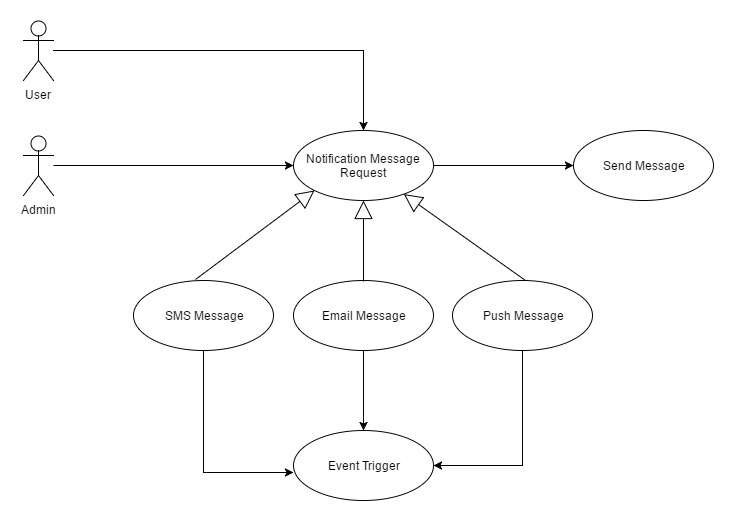
\includegraphics[width=0.7\textwidth]{notification/img/NotificationUseCase.jpg}
	\caption{Notification core functionality }
\end{figure}
